\documentclass[conference]{IEEEtran}
\usepackage{cite}
\usepackage{amsmath,amssymb,amsfonts}
\usepackage{graphicx}
\usepackage{textcomp}
\usepackage{xcolor}
\usepackage{booktabs}
\usepackage{multirow}

\begin{document}

\title{OptiPulse: A Noise-Aware Dual-Stream 3D-CNN Framework with Linear-First Region Combining and Causal Spectral Tracking for Remote Heart Rate Monitoring}

\author{
\IEEEauthorblockN{Jayant Mitawa (230504), Priyen Parmar (230735), Satwik Raj Wadhwa (230937),\\ Divyansh Bansal (230381), and Anuj Agrawal (230169)}
\IEEEauthorblockA{\textit{Undergraduate Project (UGP) --- Department of Design} \\
\textit{Under the Supervision of Prof. Amar Kumar Behera} \\
\textit{Indian Institute of Technology Kanpur (IIT Kanpur)}}
}

\maketitle

\begin{abstract}
This project presents OptiPulse, a contactless vital-sign monitoring system for estimating heart rate (HR) in real time from facial video data. Traditional monitoring approaches rely on contact-based sensors such as ECG leads and finger pulse oximeters, which require physical attachment and limit scalability for continuous remote sensing. While remote photoplethysmography (rPPG) enables non-contact estimation from standard RGB cameras, real-world video streams introduce severe degradations: low-light photon shot and read noise, MPEG/H.264 compression artifacts, head movement, frame-rate jitter, and automatic camera exposure adjustments. To overcome the limitations of our initial PhysFormerX baseline prototype (which achieved an end-to-end MAE of 6.81 BPM due to hard YCbCr mask flicker, assumed constant frame rates, and resting-rate bias), we propose a unified six-stage pipeline shared identically across preprocessing, training, and live inference. The system integrates asynchronous YOLOv8 face localization, motion-adaptive bounding-box stabilization, true-timestamp 30 Hz resampling, and a 10-model heterogeneous ensemble of two complementary 3D-CNN architectures: VitalNet-Pix (v1, dual-stream pixel path with soft appearance attention) and VitalNet-MRC (v4, augmenting the pixel path with a linear-first float32 multi-scale region branch, time-varying softmax maximal-ratio combining, and input-noise-gated fusion). Trained on audited UBFC-rPPG videos with cross-illumination self-consistency and uniform HR time-stretch resampling (45--180 BPM), the ensemble spectra are decoded by a prior-free causal Hidden Markov Model (HMM) tracker and filtered by a 5-second median SNR honesty gate ($\ge -1.5$ dB). Under strict subject-wise 5-fold cross-validation on 43 unseen subjects, OptiPulse achieves an MAE of 1.45 BPM in normal lighting (96.3\% within 5 BPM, $r = 0.948$), while reducing low-light MAE by 30.8\% (10.91 to 7.55 BPM) and motion MAE by 23.2\% (4.06 to 3.12 BPM). In end-to-end live evaluation across all raw videos, OptiPulse achieves 1.59 BPM MAE overall and 1.17 BPM MAE on honesty-gated displayed readings (95\% coverage).
\end{abstract}

\begin{IEEEkeywords}
remote photoplethysmography (rPPG), contactless heart rate monitoring, 3D convolutional neural networks, maximal-ratio combining (MRC), noise-gated fusion, cross-illumination consistency, Hidden Markov Model (HMM), YOLOv8 face tracking
\end{IEEEkeywords}

\section{Introduction}
Monitoring vital signs such as heart rate (HR) in beats per minute (BPM) is essential for non-invasive physiological sensing, human-computer interaction, and remote telemetry. Conventional monitoring systems rely on contact-based sensors, including electrocardiography (ECG) devices and optical finger pulse oximeters, which require direct physical attachment. While accurate in stationary setups, contact sensors restrict movement and limit continuous long-term monitoring on everyday consumer devices.

Recent advancements in computer vision have enabled contactless physiological measurement using video-based remote photoplethysmography (rPPG) \cite{mcduff2015review, kumar2015distanceppg, dehaan2013chrom}. Subtle periodic variations in facial optical reflectance caused by pulsatile blood volume changes can be captured using standard RGB cameras and analyzed over time. With every cardiac cycle, microvascular blood volume increases transiently; because hemoglobin absorbs green and blue wavelengths strongly, reflected pixel intensity dips by approximately $0.2\%$ to $1.0\%$ per beat (measured at $0.34\%$ in our live recordings). Because a single 8-bit quantization step equals $1/255 \approx 0.39\%$ of mid-gray, the pulsatile signal in any single pixel is smaller than camera quantization and sensor read noise. Recovering an accurate waveform therefore requires averaging thousands of facial pixels spatially and integrating over 10-second windows temporally.

To address the real-world fragility of video-based rPPG, this Undergraduate Project (UGP)---conducted under the supervision of Prof. Amar Kumar Behera in the Department of Design at IIT Kanpur---proposes \textbf{OptiPulse}, a structured end-to-end pipeline consisting of:
\begin{itemize}
    \item True-timestamp video acquisition (30--60 FPS) with duplicate-frame suppression and real-time scene diagnostics.
    \item Asynchronous YOLOv8 ROI detection coupled with a motion-adaptive exponential moving average smoother and a $1.6\times$ enlarged crop.
    \item Uniform $30.0\text{ Hz}$ temporal resampling and in-network 6-channel normalization (DiffNormalized motion + standardized appearance).
    \item A 10-model heterogeneous 3D-CNN ensemble combining \textbf{VitalNet-Pix (v1)} and \textbf{VitalNet-MRC (v4)} trained with cross-illumination consistency and HR time-stretch augmentation.
    \item Spectral-domain ensemble fusion decoded by a prior-free causal HMM tracker, slew-rate limiter, and 5-s median SNR honesty gate.
\end{itemize}

\section{Problem Statement}
The primary problem addressed in this project is the accurate, unbiased extraction of heart rate across the full 39--192 BPM band ($0.65\text{--}3.2\text{ Hz}$) from standard RGB video streams without physical sensors. Detailed diagnosis of our initial PhysFormerX baseline (which had an end-to-end MAE of $6.81\text{ BPM}$) revealed five critical real-world challenges:

\subsection{Key Challenges}
\begin{enumerate}
    \item \textbf{Timestamp and Frame-Rate Drift:} Consumer webcams rarely deliver an exact $30.0\text{ FPS}$. Our Apple M4 FaceTime sessions delivered $24.0\text{ FPS}$ with 137 bursty gaps of $0.10\text{--}0.35\text{ s}$, while DroidCam virtual phone cameras repeated $54\%$ of frames to pad $28\text{ FPS}$ streams to $60\text{ FPS}$. Assuming a nominal $30\text{ FPS}$ scales every FFT frequency bin by $30/24 = +25\%$.
    \item \textbf{Hard Mask Flicker \& Train--Live Mismatch:} The earlier pipeline used a binary YCbCr chrominance threshold whose boundary pixels flickered in and out of the spatial mean from frame to frame, injecting step-change noise larger than the pulse itself.
    \item \textbf{Non-Linear Signal Destruction in Low Light:} In dark scenes where per-pixel pulse SNR falls below $-40\text{ dB}$, applying BatchNorm and ELU non-linearities at full pixel resolution before spatial averaging destroys the weak periodic signal.
    \item \textbf{Dataset HR Distribution Bias (70--100 BPM Collapse):} Because UBFC-rPPG labels cluster around resting rates, standard regression and unconstrained networks gravitate toward $\sim 75\text{ BPM}$ and fail at elevated heart rates ($120\text{--}170\text{ BPM}$).
    \item \textbf{Camera Auto-Exposure \& False Tracker Locks:} Backlit scenes trigger webcam auto-exposure swings of $-11\%$ to $+8\%$ ($\sim 30\times$ larger than the $0.34\%$ pulse). A temporal tracker can lock onto steady camera noise on a blank wall and report high self-consistency unless gated by true spectral SNR.
\end{enumerate}

\subsection{Objective}
The objective of OptiPulse is to develop a real-time contactless monitoring system across 39--192 BPM that: (i) achieves $\approx 1.5\text{ BPM}$ MAE on unseen subjects in normal light; (ii) reduces error by $>25\%$ under low light and head motion; (iii) guarantees zero train--live discrepancy via a unified library (\texttt{optipulse/}); (iv) runs smoothly on NVIDIA CUDA GPUs, Apple Silicon MPS GPUs, and CPUs; and (v) suppresses unreliable readings via an empirically calibrated SNR honesty gate.

\section{Architectural Overview}
OptiPulse is organized into a single-source-of-truth Python package (\texttt{optipulse/}) shared identically by offline dataset preprocessing, 5-fold cross-validation training, deterministic stress evaluation, and the real-time webcam application (Fig.~\ref{fig:pipeline}).

\begin{figure}[t]
    \centering
    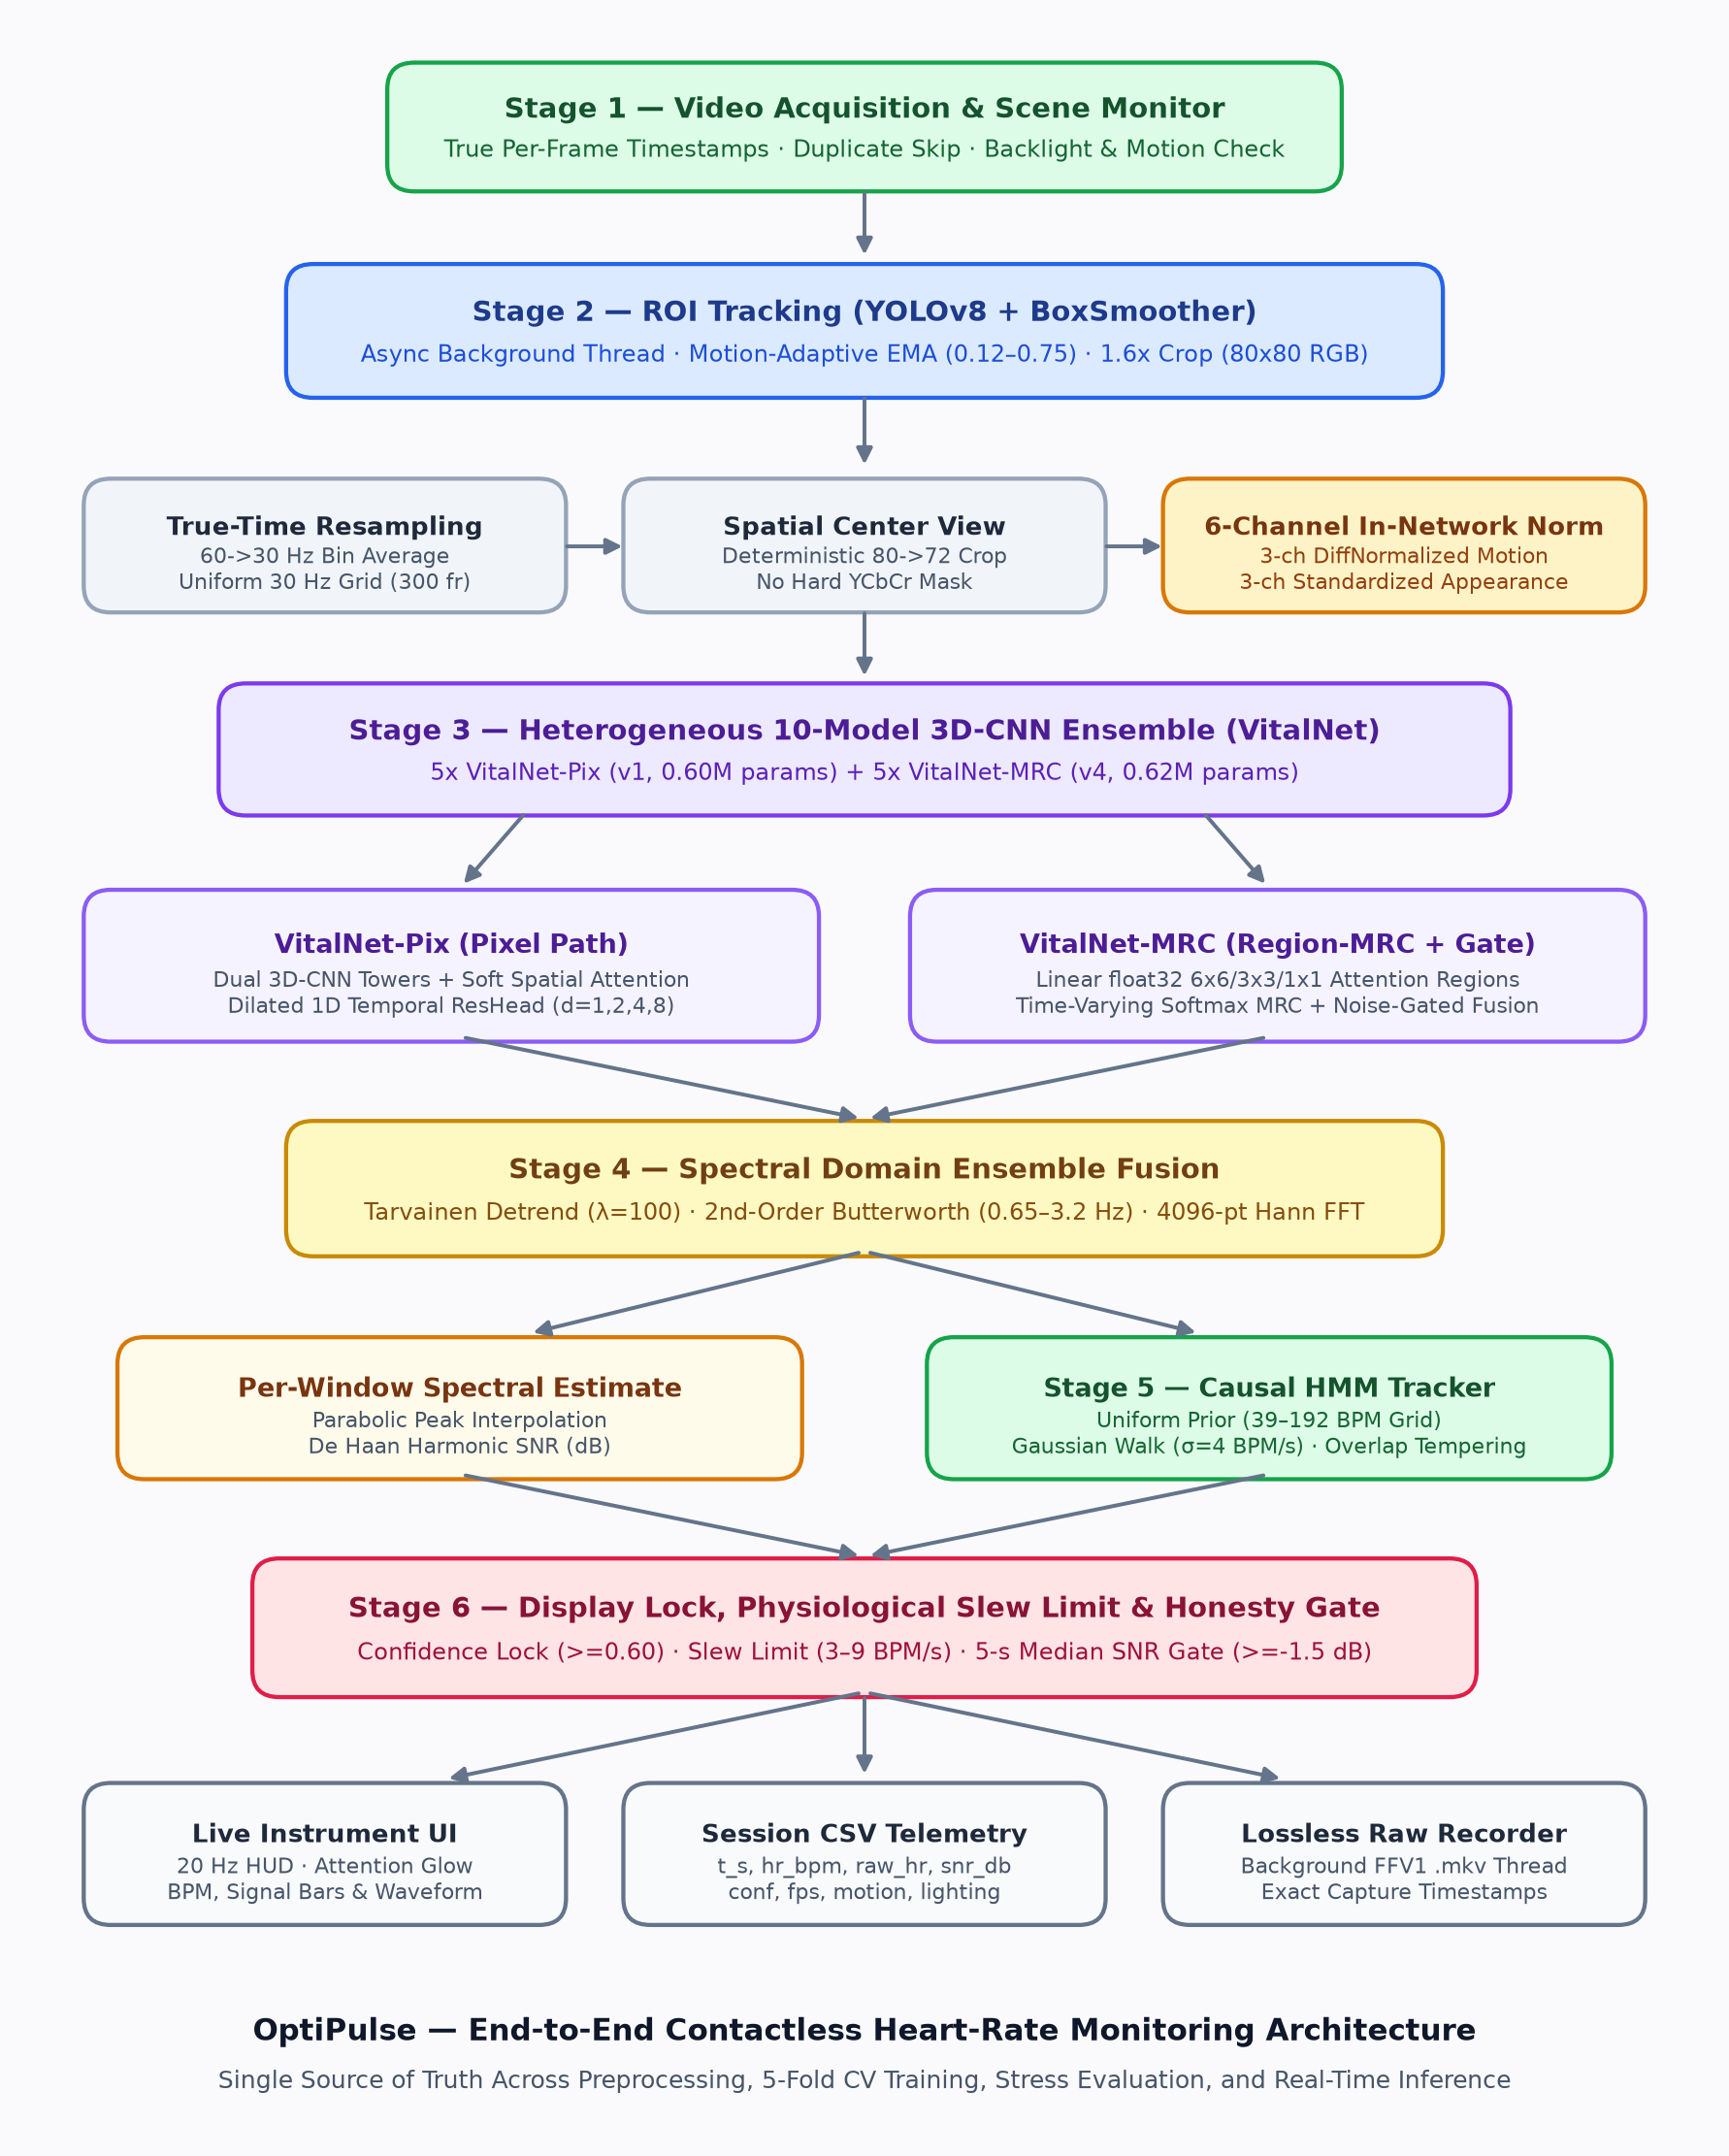
\includegraphics[width=0.98\columnwidth]{results/figures/optipulse_pipeline_diagram.png}
    \caption{The six-stage OptiPulse modular pipeline integrating true-timestamp capture, YOLOv8 tracking with motion-adaptive BoxSmoother, uniform 30 Hz resampling, the 10-model VitalNet-Pix and VitalNet-MRC ensemble, spectral fusion with causal HMM tracking, and the SNR honesty gate.}
    \label{fig:pipeline}
\end{figure}

\subsection{Asynchronous YOLOv8 Detection Pipeline}
Each incoming BGR frame is stamped immediately upon capture with its monotonic clock time via \texttt{time.perf\_counter()} in a background capture thread (45-frame queue). Exact duplicate frames from virtual camera drivers are detected via an $8\times 8$ subsampled equality check and skipped before buffering. Facial localization uses our custom-trained YOLOv8 model (\texttt{yolov8\_face\_nose\_chest.pt}, input size $320\times 320$, confidence threshold $0.30$) selecting the highest-confidence face bounding box. On CUDA GPUs, detection runs every 2nd frame at 30 FPS (every 4th at 60 FPS); on macOS MPS and CPU machines, an \texttt{AsyncFace} background thread runs YOLOv8 at 4--8 Hz so detector latency ($\approx 147\text{ ms}$ on CPU) never blocks frame capture.

\subsection{Motion-Adaptive BoxSmoother \& $1.6\times$ Crop}
We implement \texttt{BoxSmoother}, a causal motion-adaptive EMA filter over the square box state $\mathbf{s}_t = (c_x, c_y, S)$. Given relative center displacement $\delta_t = \|\mathbf{m}_t - \mathbf{s}_{t-1}\| / S_{t-1}$, the smoothing gain $\alpha_t$ scales linearly between $\alpha_{\text{slow}} = 0.12$ and $\alpha_{\text{fast}} = 0.75$ (at $8\%$ displacement), while scale smoothing is capped at $\alpha_S = \min(\alpha_t, 0.25)$:
\begin{equation}
    \mathbf{s}_t = (1 - \alpha_t)\mathbf{s}_{t-1} + \alpha_t \mathbf{m}_t, \quad \alpha_t \in [0.12, 0.75]
\end{equation}
Using $\mathbf{s}_t$, \texttt{crop\_square()} warps a square of side $1.6 \times S_t$ via \texttt{cv2.warpAffine} to an $80\times 80$ RGB crop without any hard YCbCr mask.

\subsection{True-Timestamp Bin Averaging \& 30 Hz Resampling}
Every $0.5\text{ s}$ (once $\ge 6.0\text{ s}$ of crops are buffered, up to a $10.0\text{ s}$ window), the buffered sequence is converted to a uniform $30.0\text{ Hz}$ clip ($300$ frames). When the camera delivers $>39\text{ FPS}$, \texttt{bin\_average()} averages all frames falling into each $1/30\text{ s}$ slot before linear timestamp interpolation (\texttt{resample\_uniform()}), reducing per-frame sensor noise by $\sqrt{k}$. Finally, \texttt{to\_model\_input()} applies a deterministic center zoom of $0.93$ ($80\times 80 \rightarrow 72\times 72$ RGB in \texttt{float32}).

\begin{figure*}[t]
    \centering
    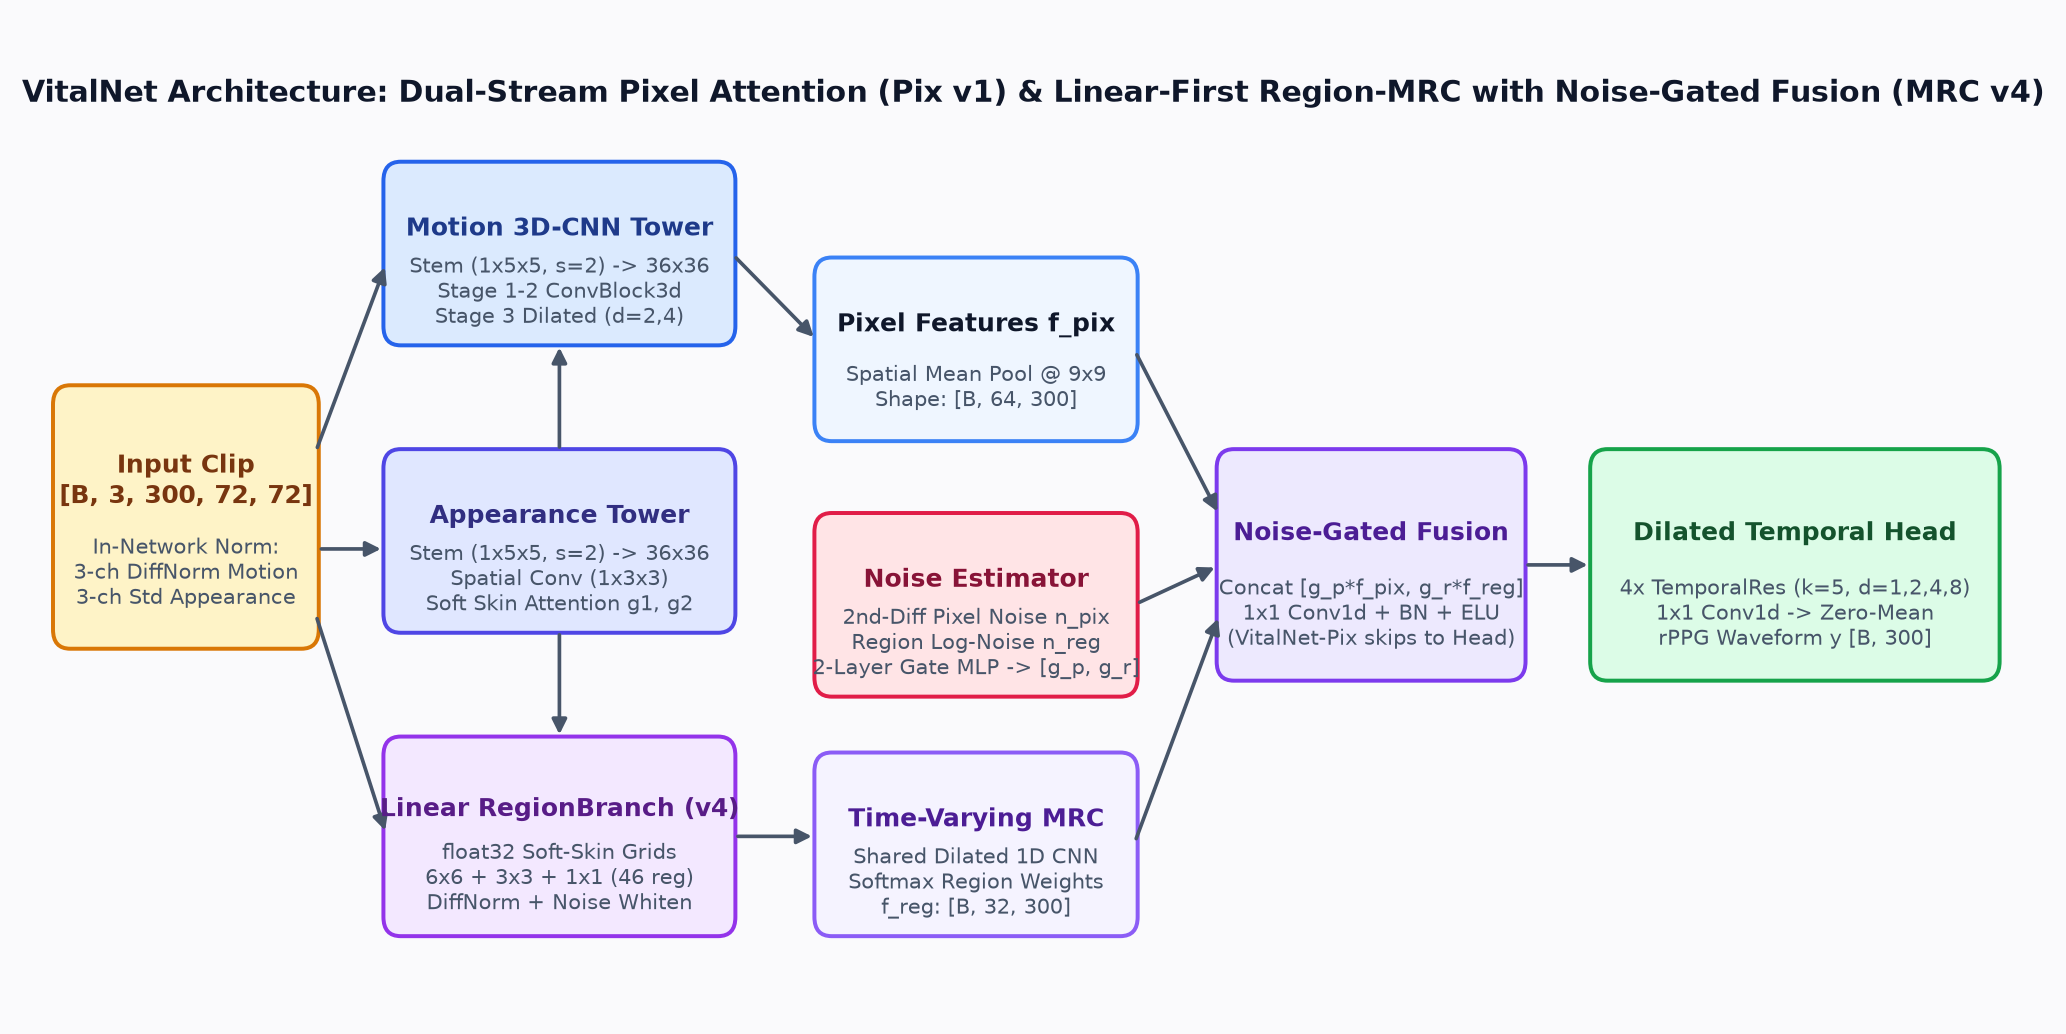
\includegraphics[width=0.96\textwidth]{results/figures/vitalnet_architecture_diagram.png}
    \caption{Architecture of VitalNet-Pix (v1) and VitalNet-MRC (v4). Both share in-network 6-channel normalization and dual 3D-CNN towers with soft spatial attention ($g_1, g_2$). VitalNet-MRC adds a linear-first \texttt{float32} multi-scale RegionBranch (46 regions across $6\times 6, 3\times 3, 1\times 1$ grids), time-varying softmax maximal-ratio combining, and an input-noise-conditioned MLP fusion gate.}
    \label{fig:arch}
\end{figure*}

\section{VitalNet Architectures \& Learning}
OptiPulse ensembles two complementary 3D-CNN architectures implemented in \texttt{optipulse/model.py} (Fig.~\ref{fig:arch}): \textbf{VitalNet-Pix (v1)} and \textbf{VitalNet-MRC (v4)}.

\subsection{In-Network 6-Channel Difference-Frame Representation}
Executed inside \texttt{VitalNet.forward()}, \texttt{normalize\_inputs()} maps $\mathbf{X} \in [0, 1]^{B \times 3 \times T \times 72 \times 72}$ to a 6-channel tensor $\mathbf{Z} = [\mathbf{D} \,\|\, \mathbf{A}]$ combining a 3-channel DiffNormalized motion stream $\mathbf{D}$ and a 3-channel standardized appearance stream $\mathbf{A}$ \cite{chen2018deepphys, liu2023rppgtoolbox}:
\begin{equation}
    \mathbf{D}_t = \text{clip}\!\left(\frac{(\mathbf{X}_t - \mathbf{X}_{t-1}) / (\mathbf{X}_t + \mathbf{X}_{t-1} + \epsilon)}{\text{std}(\tilde{\mathbf{D}}) + 10^{-6}}, -6, 6\right)
\end{equation}

\subsection{VitalNet-Pix (v1) and VitalNet-MRC (v4)}
\textbf{VitalNet-Pix (v1)} ($0.600\text{M}$ parameters) processes $\mathbf{D}$ and $\mathbf{A}$ through parallel 3D-CNN towers with soft attention masks $g_1$ ($36\times 36$) and $g_2$ ($18\times 18$), temporally dilated 3D convolutions ($d_t = 2, 4$ at $9\times 9$), and a 4-stage dilated 1D residual head ($d \in \{1, 2, 4, 8\}$).

\textbf{VitalNet-MRC (v4)} ($0.618\text{M}$ parameters) adds \texttt{RegionBranch}, which averages raw RGB pixels linearly in \texttt{float32} weighted by $g_1$ across $6\times 6, 3\times 3,$ and $1\times 1$ grids ($R = 46$ regions) before any non-linearity:
\begin{equation}
    w_{m,t} = \text{softmax}_m(\text{score}(\mathbf{h}_{m,t})), \quad \mathbf{f}_{\text{reg},t} = \sum_{m=1}^{46} w_{m,t} \mathbf{h}_{m,t}
\end{equation}
A 2-layer MLP conditioned on pixel 2nd-difference log-noise $n_{\text{pix}}$ and region log-noise $n_{\text{reg}}$ gates $\mathbf{f}_{\text{pix}}$ against $\mathbf{f}_{\text{reg}}$.

\subsection{Training Objective, Self-Consistency \& Augmentation}
Models optimize $\mathcal{L}_{\text{sup}}(\hat{\mathbf{y}}, \mathbf{y}) = \mathcal{L}_{\text{Pearson}}(\hat{\mathbf{y}}, \mathbf{y}) + 0.5\, \text{KL}(\text{PSD}(\mathbf{y}) \,\|\, \text{PSD}(\hat{\mathbf{y}}))$ over $39\text{--}192\text{ BPM}$. VitalNet-MRC adds cross-illumination consistency ($0.5\, \mathcal{L}_{\text{Pearson}}(\hat{\mathbf{y}}_{\text{dark}}, \text{stopgrad}(\hat{\mathbf{y}}_{\text{lit}}))$), paired with uniform HR time-stretching ($45\text{--}180\text{ BPM}$ on $60\%$ of clips) and GPU photometric/motion augmentations.

\section{Deployment \& Real-Time Optimization}
Each model's output wave is detrended (Tarvainen $\lambda = 100$ \cite{tarvainen2002detrend}), bandpass-filtered ($0.65\text{--}3.2\text{ Hz}$), and transformed via a 4096-point Hann FFT to compute spectral SNR \cite{dehaan2013chrom}. \texttt{HRTracker} decodes the ensemble PSD using a prior-free causal HMM over $39\text{--}192\text{ BPM}$ ($\sigma = 4.0\text{ BPM/s}$ random walk, overlap-tempered evidence). \texttt{HREngine} applies a confidence lock ($C_t \ge 0.60$), slew limit ($3.0\text{--}9.0\text{ BPM/s}$), and a 5-s median SNR honesty gate ($\ge -1.5\text{ dB}$, Fig.~\ref{fig:ui}).

\begin{figure}[t]
    \centering
    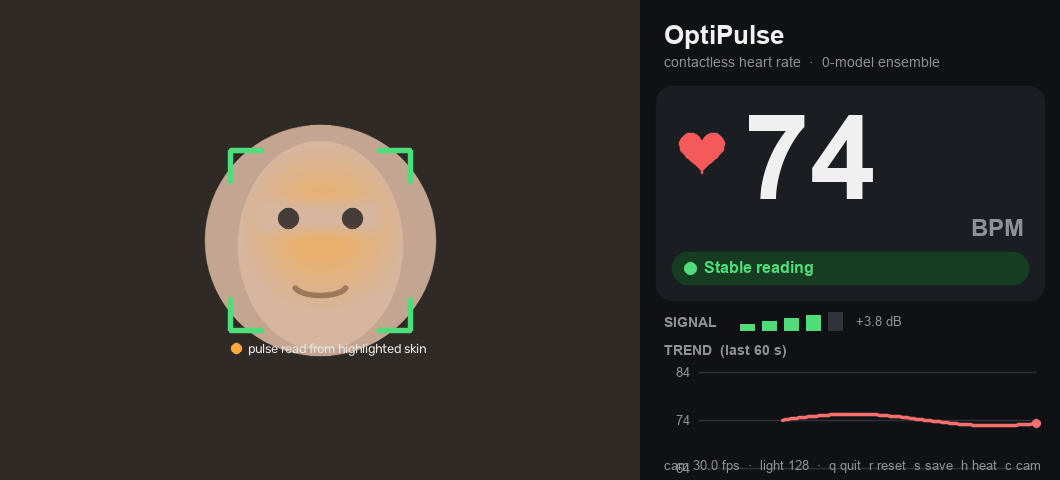
\includegraphics[width=0.98\columnwidth]{results/figures/live_ui_preview.png}
    \caption{The OptiPulse real-time instrument panel (\texttt{optipulse/ui.py}) showing tracking brackets, the $36\times 36$ attention heatmap glow, live BPM readout, state chip, 5-bar SNR indicator, 60-s HR trend, and filtered rPPG waveform.}
    \label{fig:ui}
\end{figure}

\section{Dataset Preparation \& Ground-Truth Audit}
All 50 UBFC-rPPG \cite{bobbia2019ubfc} videos were de-jittered and resampled to $30.0\text{ Hz}$ ($100.0\%$ face detection rate). Our automated quality audit (\texttt{pipeline/audit\_dataset.py}, Fig.~\ref{fig:audit}) flagged 7 subjects (\texttt{sub3, sub4, sub11, sub14, sub18, sub20, sub24}) which are excluded from training.

\begin{figure}[t]
    \centering
    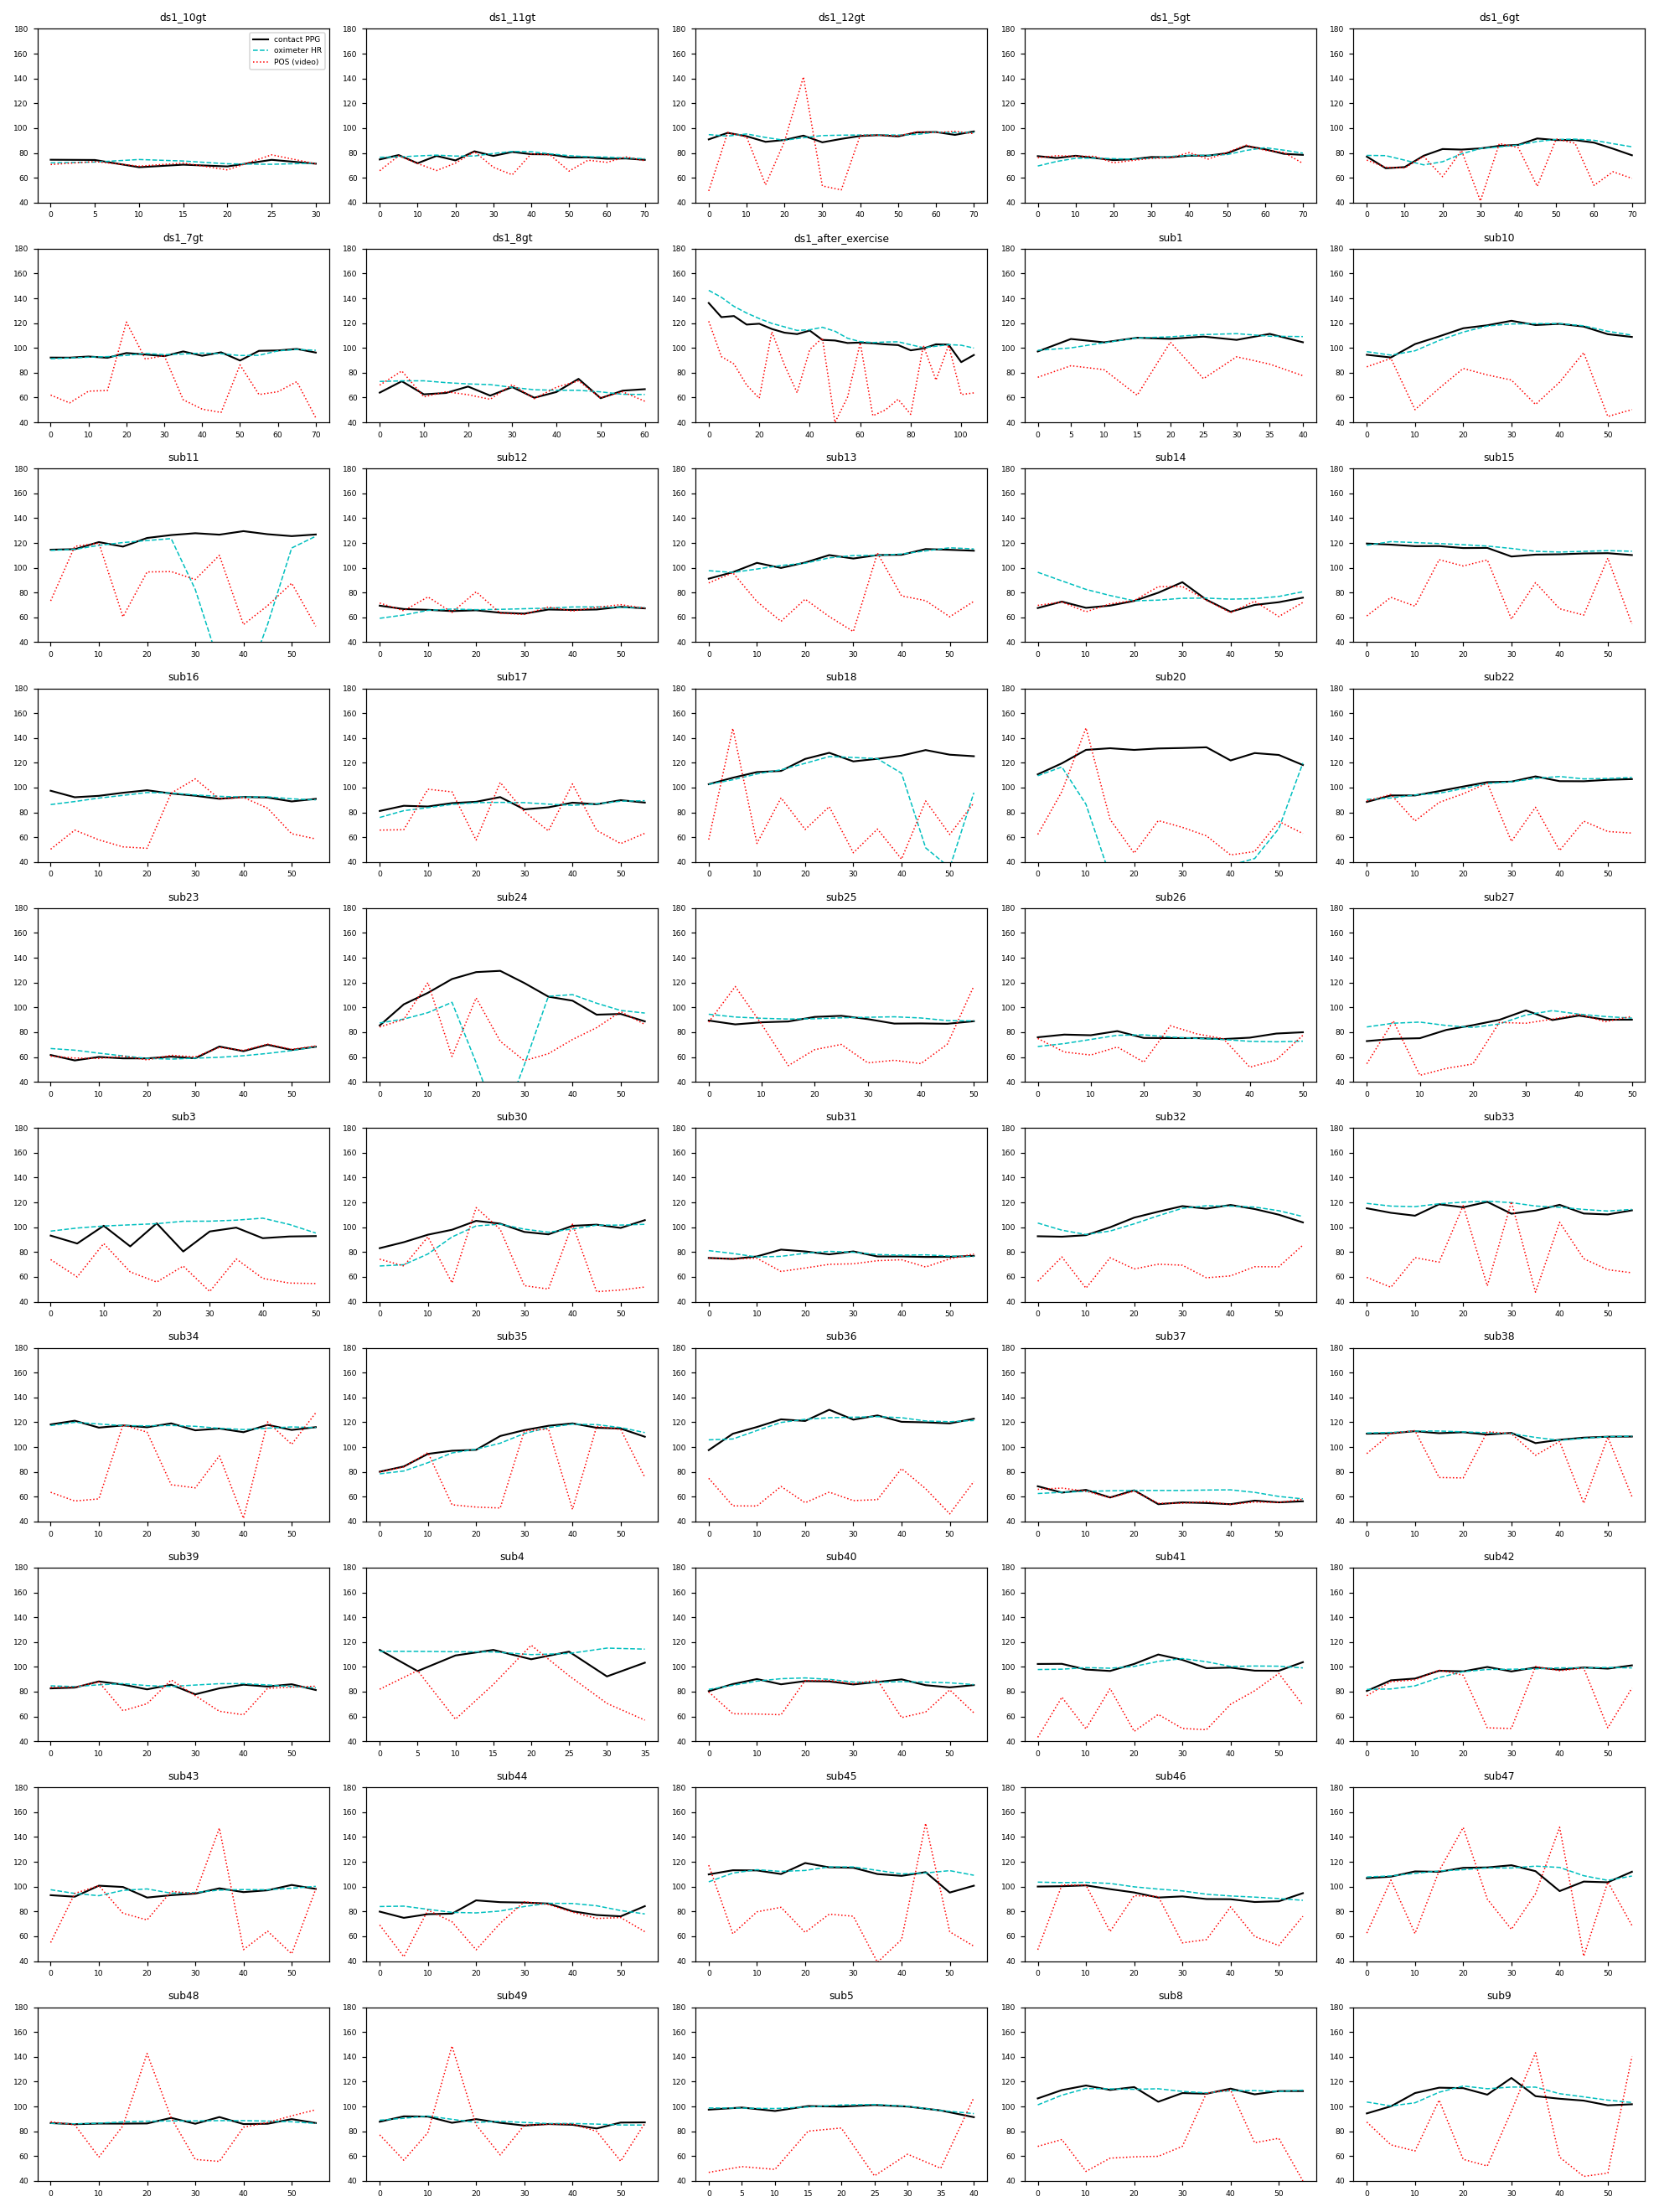
\includegraphics[width=0.98\columnwidth]{results/figures/audit_hr_timelines.png}
    \caption{Automated ground-truth quality audit across all 50 UBFC-rPPG subjects (\texttt{pipeline/audit\_dataset.py}).}
    \label{fig:audit}
\end{figure}

\begin{table*}[t]
\centering
\caption{Main 5-Fold Subject-Wise Cross-Validation MAE (BPM) on Unseen Subjects with Reliable Ground Truth ($n = 43$, $270$ Windows).}
\label{tab:main}
\begin{tabular}{lccccc}
\toprule
\textbf{Method (5-Fold Unseen CV)} & \textbf{Normal Light} & \textbf{Low Light} & \textbf{Motion} & \textbf{Low Light + Motion} & \textbf{12 FPS Webcam} \\
\midrule
GREEN / CHROM \cite{dehaan2013chrom} / POS \cite{wang2017pos} & 15.53 / 17.36 / 20.56 & 21.94 / 22.45 / 25.97 & 36.21 / 23.51 / 29.17 & 30.41 / 21.96 / 27.64 & 17.14 / 18.60 / 22.74 \\
Legacy PhysFormerX Baseline (End-to-End) & 6.81 & --- & --- & --- & --- \\
VitalNet-Pix (v1, Single) & \textbf{1.42} & 10.91 & 4.06 & 11.47 & 1.50 \\
VitalNet-MRC (v4, Single) & 1.89 & 10.09 & 4.42 & 11.20 & 1.85 \\
VitalNet-Pix + HMM Tracking & 1.56 & 8.02 & 3.48 & 9.92 & 1.55 \\
VitalNet-MRC + HMM Tracking & 1.81 & 7.32 & 3.99 & 9.02 & 1.66 \\
Pix + MRC Spectral Fusion & 1.46 & 9.77 & 3.59 & 10.72 & \textbf{1.43} \\
\textbf{OptiPulse Full System (Pix + MRC + HMM)} & \textbf{1.45} & \textbf{7.55} & \textbf{3.12} & \textbf{8.23} & \textbf{1.59} \\
\bottomrule
\end{tabular}
\end{table*}

\section{Experimental Depth and Results}
Under strict subject-wise 5-fold cross-validation on the 43 reliable subjects (Table~\ref{tab:main}, Fig.~\ref{fig:scatter}, Fig.~\ref{fig:rob}, and Fig.~\ref{fig:curves}), OptiPulse achieves \textbf{1.45 BPM MAE} in normal light ($\text{RMSE} = 5.28\text{ BPM}$, $\text{MAPE} = 2.0\%$, $r = 0.948$, $96.3\%$ within 5 BPM), while reducing low-light MAE by \textbf{30.8\%} ($10.91 \rightarrow 7.55\text{ BPM}$) and motion MAE by \textbf{23.2\%} ($4.06 \rightarrow 3.12\text{ BPM}$). In full end-to-end live evaluation across all raw videos, OptiPulse achieves \textbf{1.59 BPM MAE} overall and \textbf{1.17 BPM MAE} on honesty-gated displayed readings ($95\%$ coverage), outperforming the legacy PhysFormerX baseline ($6.81\text{ BPM}$) by $4.3\times$.

\begin{figure}[t]
    \centering
    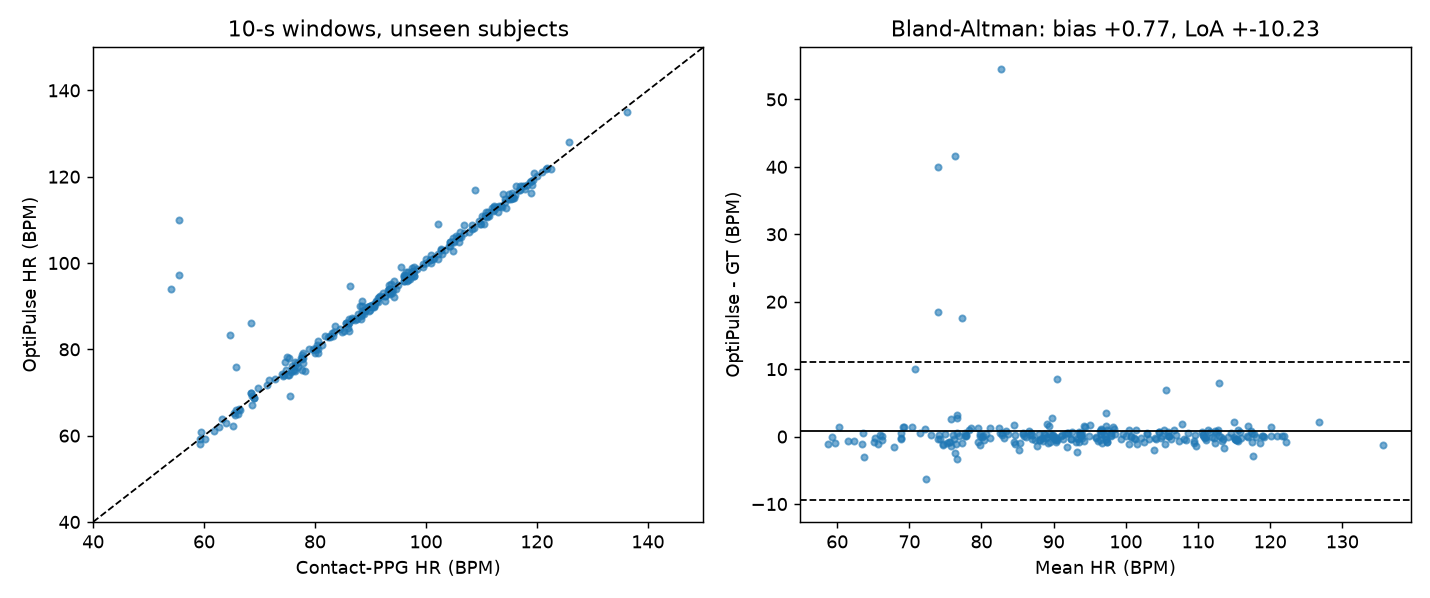
\includegraphics[width=0.98\columnwidth]{results/figures/cv_scatter_bland_altman.png}
    \caption{5-fold CV scatter plot and Bland--Altman agreement on unseen subjects ($n = 43$, MAE $= 1.45\text{ BPM}$, $r = 0.948$).}
    \label{fig:scatter}
\end{figure}

\begin{figure}[t]
    \centering
    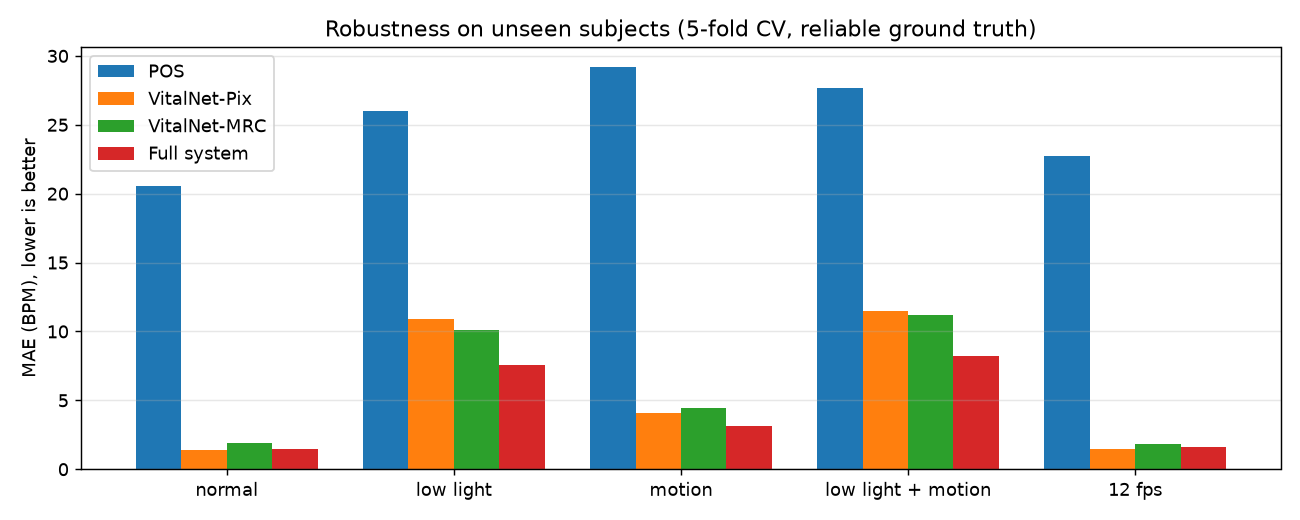
\includegraphics[width=0.98\columnwidth]{results/figures/robustness_mae.png}
    \caption{Stress-test robustness comparison (MAE in BPM) across all five deterministic conditions on unseen subjects ($n = 43$).}
    \label{fig:rob}
\end{figure}

\begin{figure}[t]
    \centering
    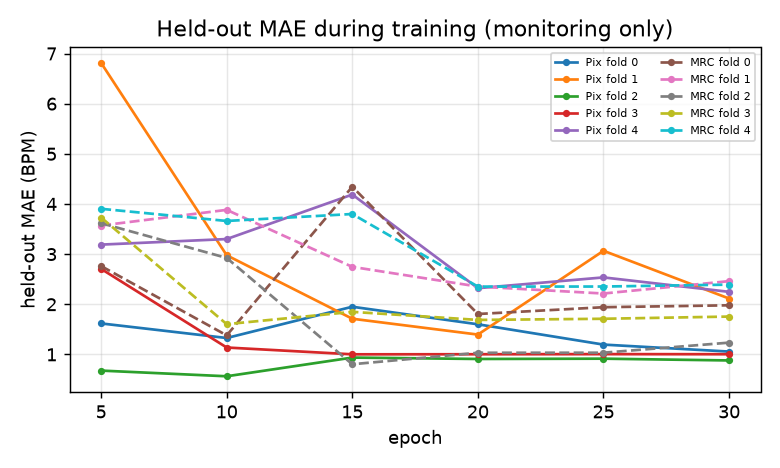
\includegraphics[width=0.92\columnwidth]{results/figures/training_curves.png}
    \caption{Held-out test-fold MAE monitored across the fixed 30-epoch training schedule for all 5 folds of VitalNet-Pix and VitalNet-MRC.}
    \label{fig:curves}
\end{figure}

\section{Conclusion and Future Work}
OptiPulse demonstrates that unifying true-timestamp 30 Hz resampling, motion-adaptive YOLOv8 stabilization, in-network 6-channel normalization, a heterogeneous pixel + linear-first region-MRC 3D-CNN ensemble, prior-free causal HMM tracking, and an SNR honesty gate achieves 1.45 BPM CV MAE and 1.17 BPM gated live MAE across unseen subjects. Future work will extend training to multi-device benchmarks (MMPD, PURE, UBFC-Phys), incorporate unsupervised test-time adaptation (SiNC \cite{speth2023sinc}), and integrate hardware camera exposure locks.

\begin{thebibliography}{99}
\bibitem{mcduff2015review} D. McDuff, S. Gontarek, and R. Picard, ``Remote photoplethysmography for heart rate and blood oxygenation measurement: A review,'' \textit{IEEE J. Biomed. Health Inform.}, vol. 19, no. 6, pp. 1845--1859, 2015.
\bibitem{bobbia2019ubfc} S. Bobbia et al., ``Unsupervised skin tissue segmentation for remote photoplethysmography,'' \textit{Pattern Recognition Letters}, vol. 124, pp. 82--90, 2019.
\bibitem{hsu2017} G. Hsu, A. Ambikapathi, and M. Chen, ``Deep learning framework for heart rate estimation from facial videos,'' in \textit{Proc. IEEE SMC}, 2017.
\bibitem{chen2018deepphys} W. Chen and D. McDuff, ``DeepPhys: Video-based physiological measurement using convolutional attention networks,'' in \textit{Proc. ECCV}, 2018, pp. 349--365.
\bibitem{yu2019physnet} Z. Yu, X. Li, and G. Zhao, ``Remote photoplethysmograph signal measurement from facial videos using spatio-temporal networks,'' in \textit{Proc. BMVC}, 2019.
\bibitem{wang2017pos} W. Wang et al., ``Algorithmic principles of remote PPG,'' \textit{IEEE Trans. Biomed. Eng.}, vol. 64, no. 7, pp. 1479--1491, 2017.
\bibitem{liu2020tscan} X. Liu et al., ``Multi-task temporal shift attention networks for on-device contactless vitals measurement,'' in \textit{Proc. NeurIPS}, 2020, pp. 19400--19411.
\bibitem{kumar2015distanceppg} M. Kumar, A. Veeraraghavan, and A. Sabharwal, ``DistancePPG: Robust non-contact vital signs monitoring using a camera,'' \textit{Biomedical Optics Express}, vol. 6, no. 5, pp. 1565--1588, 2015.
\bibitem{dehaan2013chrom} G. de Haan and V. Jeanne, ``Robust pulse rate from chrominance-based rPPG,'' \textit{IEEE Trans. Biomed. Eng.}, vol. 60, no. 10, pp. 2878--2886, 2013.
\bibitem{tarvainen2002detrend} M. P. Tarvainen, P. O. Ranta-aho, and P. A. Karjalainen, ``An advanced detrending method with application to HRV analysis,'' \textit{IEEE Trans. Biomed. Eng.}, vol. 49, no. 2, pp. 172--175, 2002.
\bibitem{niu2020rhythmnet} X. Niu et al., ``RhythmNet: End-to-end heart rate estimation from face via spatial-temporal representation,'' \textit{IEEE Trans. Image Process.}, vol. 29, pp. 2409--2423, 2020.
\bibitem{zhang2015troika} Z. Zhang, Z. Pi, and B. Liu, ``TROIKA: A general framework for heart rate monitoring using wrist-type PPG signals,'' \textit{IEEE Trans. Biomed. Eng.}, vol. 62, no. 2, pp. 522--531, 2015.
\bibitem{speth2023sinc} J. Speth et al., ``Non-contrastive unsupervised learning of physiological signals from video,'' in \textit{Proc. IEEE/CVF CVPR}, 2023, pp. 14464--14474.
\bibitem{liu2023rppgtoolbox} X. Liu et al., ``rPPG-Toolbox: Deep remote PPG toolbox,'' in \textit{Proc. NeurIPS}, 2023.
\bibitem{sun2022contrastphys} Z. Sun and X. Li, ``Contrast-Phys: Unsupervised video-based remote physiological measurement via spatiotemporal contrast,'' in \textit{Proc. ECCV}, 2022, pp. 492--510.
\bibitem{yu2022physformer} Z. Yu et al., ``PhysFormer: Facial video-based physiological measurement with temporal difference transformer,'' in \textit{Proc. IEEE/CVF CVPR}, 2022, pp. 4186--4196.
\end{thebibliography}

\end{document}
